\documentclass[acmsmall,screen]{acmart}

\setcopyright{none}
\settopmatter{printacmref=false}
\renewcommand\footnotetextcopyrightpermission[1]{}
\acmConference[Post-Mid-Semester Evaluation]{AI Tools for Research}{November 2026}{Prayagraj, India}
\acmBooktitle{AI Tools for Research -- Post-Mid-Semester Evaluation (2026)}

\usepackage{booktabs}
\usepackage{tabularx}
\usepackage{multirow}
\usepackage{enumitem}
\usepackage{xcolor}
\newcommand{\pending}[1]{\textcolor{red}{[TO VERIFY: #1]}}

\title{Is the Judge the Bottleneck?}
\subtitle{A Judge-Swap Study of Consistency-Based Detection of Fabricated References in Large Language Models}

\author{Nagireddy Nithin Kumar Reddy}
\affiliation{%
  \institution{Indian Institute of Information Technology Allahabad}
  \department{M.Tech Information Technology with Specialization in AI/ML; Roll No.: MAI2026010}
  \city{Prayagraj}
  \country{India}}
\email{mai2026010@iiita.ac.in}
\renewcommand{\shortauthors}{Nagireddy Nithin Kumar Reddy}

\begin{abstract}
Large language models (LLMs) fabricate bibliographic references, and a model's own consistency can reveal them: when asked repeatedly who wrote a reference, models tend to give stable author lists for real works and unstable ones for invented works. Agrawal et al.\ reported that such consistency checks detect hallucinated references well for GPT-4 but are ineffective for 7B--13B models, where the language model also acts as the judge of its own answers. We ask whether that failure lies in the judge or in the answers. Using the authors' released data (six models, 200 ACM computing topics, 1{,}000 references per model), we first reproduce all 36 published AUC values to within 0.0005, and in doing so find that one released file duplicates 200 references. We then run a judge-swap ablation: the same three sampled author answers per reference are scored by the original LM judge, by an external natural-language-inference (NLI) judge as used in SelfCheckGPT, and by a model-free name-overlap judge. The external NLI judge does not recover detection: on Llama-2-7B all judges remain near chance (AUROC 0.51--0.56; NLI minus LM judge $+0.046$, 95\% CI $[-0.003, 0.094]$), and on the five larger models NLI is significantly worse than the LM judge (by 0.05--0.14). The model-free overlap judge matches the LM judge everywhere and beats it on two models. This pattern is consistent with the small-model failure lying in the sampled answers rather than in the judge. On references whose Bing label is confirmed by scholarly databases, the judges remain weak (AUROC 0.54--0.61) and the NLI--LM difference is still not significant. For research workflows, a cheap name-overlap check is as informative as an LM-based one. A pre-registered familiarity analysis finds a weak, non-significant tendency for fewer fabrications on well-published topics. All code, protocol, logs and an AI-use record are released.
\end{abstract}

\keywords{hallucination detection, citation fabrication, self-consistency, SelfCheckGPT, reproduction, natural language inference, research integrity}

\ccsdesc[500]{Computing methodologies~Natural language processing}
\ccsdesc[300]{Information systems~Information retrieval}

\begin{document}
\maketitle

\section{Introduction}\label{sec:intro}
Fabricated references are one of the most consequential hallucinations in LLM-assisted research because they create an apparently traceable evidence chain. Audits have documented substantial fabrication across scientific, medical and systematic-review settings \cite{walters2023fabrication,athaluri2023exploring,bhattacharyya2023high,chelli2024hallucination}, with rates that depend on model, domain and topic familiarity \cite{linardon2025topic}. The author's earlier review of hallucination types for research applications \cite{reddy2026taxonomy} argued that citation \emph{existence} and citation \emph{support} are separate verification problems and that self-assessment by the model is an unreliable safeguard \cite{dahl2024large}. This paper takes the first of those problems and studies one detection mechanism experimentally.

Sampling-based consistency checks detect hallucinations without external resources: if a model knows a fact, repeated samples agree; if it invents it, they diverge \cite{manakul2023selfcheck}. Agrawal et al.\ showed that asking a model repeatedly about author lists works well to spot fake citations in GPT-4, but fails for smaller models like Llama-2-7B \cite{agrawal2023hallucinating}. Agrawal et al.\ already tested Llama-2 models (7B, 13B, and 70B) and found that consistency checks performed near chance on the 7B size. Their \emph{indirect query} (IQ) asks for the authors of a generated title in three independent sessions and lets the same LM judge how much the author lists overlap; their \emph{direct queries} (DQ) ask the model whether the reference exists. Because their setup used the language model itself to judge whether sampled author lists agreed, we ask \emph{why} it fails: is the issue a weak judge, or do the sampled answers themselves lack a consistency signal? To isolate this, we keep the original sampled author responses fixed and swap only the scoring judge—comparing their original LM judge against an external natural language inference (NLI) judge and a model-free string name-overlap judge.

\paragraph{Contributions}
\begin{enumerate}[leftmargin=*]
  \item A verified reproduction of all 36 AUC values reported by Agrawal et al.\ from their released scores (max.\ deviation 0.0005), with an explanation of a text--figure discrepancy and the discovery of 200 duplicated references in one released file (\S\ref{sec:baselines}).
  \item A \emph{judge-swap ablation} that keeps the sampled author answers fixed and changes only the judge (LM, external NLI, model-free name overlap) across six models from Llama-2-7B to GPT-4 (\S\ref{sec:e1}).
  \item A robustness check of the Bing-based ground truth against scholarly databases (OpenAlex, Crossref) and a pre-registered test of topic familiarity (\S\ref{sec:r1}, \S\ref{sec:rq2}).
\end{enumerate}
The main result is negative for the hypothesis we pre-registered and, we argue, informative: changing the judge does not rescue small models.

\section{Related Work}\label{sec:related}
\textbf{Hallucination taxonomies.} Surveys distinguish factuality from faithfulness and intrinsic from extrinsic errors \cite{ji2023survey,huang2025survey}; fabricated references are extrinsic, entity-level factual fabrications in that vocabulary. \textbf{Citation audits} measure fabrication by manual or database-backed checking \cite{walters2023fabrication,bhattacharyya2023high,chelli2024hallucination} and report topic dependence \cite{linardon2025topic}. \textbf{Detection without external knowledge} includes sampling consistency \cite{manakul2023selfcheck}, reference-specific consistency queries \cite{agrawal2023hallucinating}, self-evaluation of correctness \cite{kadavath2022knowledge} and semantic uncertainty \cite{kuhn2023semantic}; Kalai and Vempala argue that calibrated models must hallucinate rare facts \cite{kalai2024calibrated}. \textbf{Detection with external knowledge} decomposes text into atomic facts \cite{min2023factscore}, uses benchmarks \cite{li2023halueval,niu2024ragtruth}, or verifies references against bibliographic sources, recently with retrieval, fuzzy matching and an LLM verifier \cite{misra2026detecting}; at web scale, citation URLs produced by LLMs and deep-research agents have been audited for resolvability \cite{rao2026detecting}. Our study is closest to \cite{agrawal2023hallucinating}: we reuse its data and checks and add a controlled change of the judge, which that work did not test.

\section{Research Questions}\label{sec:rq}
\textbf{RQ1 (judge).} Holding the three sampled author answers fixed, does an external NLI judge (J-NLI) detect hallucinated references better than the LM judge (J-LM)? \emph{H1}: AUROC(J-NLI) $>$ AUROC(J-LM). The paired contrast was registered for each of the six models; the hypothesis was motivated by the small models, and Llama-2-7B is the setting closest to the registered 7B target. H1 is supported for a model if the paired 95\% CI of the difference lies above 0. Six contrasts are reported without multiplicity correction.
\textbf{RQ2 (familiarity).} Is fabrication more frequent for topics with fewer publications? \emph{H2}: the logistic slope of $P(\text{hallucinated})$ on $\log_{10}$ topic works is negative; supported for a model if its 95\% CI lies below 0.
A third question on the number of samples, and a new-generator experiment (Qwen2.5-1.5B), were planned but dropped for time before they produced results; the pipeline is released but unexecuted (\S\ref{sec:limits}).

\section{Method}\label{sec:method}
\subsection{Data}
We use the results released with \cite{agrawal2023hallucinating} (repository \texttt{microsoft/hallucinated-references}, commit \texttt{bf3ef5f}, MIT licence): for each of GPT-4, GPT-3.5-turbo, text-davinci-003 and Llama-2-Chat 7B/13B/70B, 1{,}000 generated titles (5 per topic for 200 ACM CCS topics), a Bing exact-title label (no result $\Rightarrow$ hallucinated, $y=1$), three sampled author answers, and the released IQ and DQ scores. File integrity was checked against the paper's hallucination rates (e.g.\ GPT-4 468/1{,}000 = 46.8\%, Llama-2-7B 68.3\%). The Llama-2-13B file covers only 160 topics: rows 700--899 repeat 200 (topic, title) pairs with identical labels but re-sampled answers; we deduplicate it (800 references) for all new analyses. Ten topics, drawn with a fixed seed, form a \emph{pilot} set used only to set parsing and matching rules; all reported results use the remaining 190 \emph{main} topics (5{,}520 references; 770 for 13B).

\subsection{Judges}
All judges score a reference from its three author answers $a_1,a_2,a_3$; higher means more likely hallucinated, and the orientation is fixed in advance.
\textbf{J-LM} is Agrawal et al.'s released judge: the generator rates pairwise author overlap (0--100\%), averaged over the three pairs; score $=1-$overlap.
\textbf{J-NLI} uses the SelfCheckGPT NLI checkpoint (\texttt{potsawee/deberta-v3-large-mnli}) and averages $P(\text{contradiction})$ over the six ordered pairs, encoded exactly as \texttt{SelfCheckNLI}. Agrawal's LM judge is instructed to output 0 if ``either of them is not a list of authors''; we apply the same rule, scoring pairs that involve an answer with no parseable name (typically a refusal) as 1. Without the rule two refusals entail each other and look consistent; this variant (J-NLI-raw) is reported as a sensitivity check.
\textbf{J-STR} needs no model: $1-$mean pairwise Jaccard similarity of the sets of normalised name tokens. Token sets (rather than surnames) make ``Bishop, Christopher'' and ``Christopher M.\ Bishop'' agree. The parser was developed on pilot answers from the same six models (pilot topics are excluded from every result) and every rule is covered by a unit test built from real pilot rows; part of J-STR's performance may reflect this tuning.

\subsection{Baseline validation}
\textbf{V2} recomputes Agrawal's IQ, DQ1--3, DQ-ensemble and IQ+DQ AUCs from the released scores. Their figures report the mean AUC over 100 bootstrap resamples (\texttt{roc-utils}, seed 42) with an automatic flip of below-chance predictors; because that package no longer imports with current SciPy, we reimplemented its procedure. The flip is used for V2 only. \textbf{V1} reproduces SelfCheckGPT on its WikiBio benchmark (238 passages, 20 samples each).

\subsection{Ground-truth robustness (R1)}
Bing labels date from 2023 and match any web page containing the exact phrase. We re-label the Llama-2-7B main-set titles by querying OpenAlex and then Crossref (five candidates each) and calling a title \emph{found} if the best normalised similarity (\texttt{rapidfuzz} \texttt{ratio}) is $\ge 90$, \emph{partial} in $[75,90)$, else \emph{not found}. Both the threshold and the order-sensitive similarity were chosen on pilot titles: an order-insensitive measure matched a reordered fake title, and the chosen setting reached Cohen's $\kappa=0.82$ (GPT-4) and $0.80$ (Llama-2-7B) with Bing on the pilot.

\subsection{Familiarity (RQ2)}
Topic familiarity is $\log_{10}(1+n)$, where $n$ is the OpenAlex works count for the topic's leaf phrase (e.g.\ ``Topology'' in ``Continuous mathematics: Topology''). Tertiles are defined over topics, so all models share cut points.

\subsection{Statistics and protocol}
AUROC is the primary metric. CIs are 95\% percentile intervals from 2{,}000 bootstrap resamples of \emph{topics} (references within a topic are not independent); judge differences are paired, using the same resamples. No auto-flip is applied. Settings, hypotheses, decision rules and seeds were frozen before any main-set score was computed (git tag \texttt{protocol-v1}); five later changes are logged with their reasons and whether results had been seen. Three preceded all main-set results; E1 was complete when the new-generator experiment was dropped for time and when RQ2 was re-registered on the released data, and both changes record this.

\section{Results}\label{sec:results}
\subsection{Baseline validation}\label{sec:baselines}
\textbf{V2.} All 36 published values were reproduced within the pre-registered tolerance of $\pm0.005$; the maximum deviation is 0.0005. No predictor was auto-flipped, so the V2 values and our unflipped E1 values are on the same scale. Table~\ref{tab:v2} shows a subset. The paper's text quotes GPT-4 IQ 0.878 and DQ1 0.887 while its figure shows 0.877 and 0.885; our point AUCs (0.8781, 0.8868) and bootstrap means (0.8768, 0.8854) show that the text reports point estimates and the figure bootstrap means. During baseline verification, we identified 200 repeated rows in the released Llama-2-13B file. Removing these duplicate references shifted the 13B V2 AUCs by at most 0.006, demonstrating that automated test suites caught a dataset bug that ultimately did not alter the study's primary conclusions.

\begin{table}[t]
\caption{V2: published AUCs of Agrawal et al.\ (figures 5 and 9) vs.\ our recomputation from the released scores (bootstrap mean). All 36 cells, including DQ1--3, are within 0.0005 (\texttt{results/v2\_agrawal\_auc.csv}).}
\label{tab:v2}
\small
\begin{tabular}{lcccccc}
\toprule
& \multicolumn{2}{c}{IQ} & \multicolumn{2}{c}{DQ ensemble} & \multicolumn{2}{c}{IQ+DQ} \\
Model & published & ours & published & ours & published & ours \\
\midrule
GPT-4 & 0.877 & 0.8768 & 0.915 & 0.9149 & 0.927 & 0.9274 \\
GPT-3.5-turbo & 0.782 & 0.7818 & 0.624 & 0.6239 & 0.792 & 0.7922 \\
text-davinci-003 & 0.695 & 0.6947 & 0.621 & 0.6211 & 0.710 & 0.7104 \\
Llama-2-70B & 0.658 & 0.6577 & 0.658 & 0.6583 & 0.702 & 0.7020 \\
Llama-2-13B & 0.657 & 0.6568 & 0.696 & 0.6961 & 0.723 & 0.7235 \\
Llama-2-7B & 0.517 & 0.5172 & 0.573 & 0.5729 & 0.575 & 0.5747 \\
\bottomrule
\end{tabular}
\end{table}

\textbf{V1.} SelfCheck-Unigram (max) reproduces the published WikiBio results almost exactly: non-factual AUC-PR 85.64 vs.\ 85.63, factual 58.50 vs.\ 58.47, passage-level Pearson correlation 64.72 vs.\ 64.71 (all 1{,}908 sentences). The full NLI benchmark (38{,}160 premise--hypothesis pairs) was not re-run: on the available hardware it would have taken about 40\,h. Instead we verified that our batched NLI scorer is numerically identical to the official \texttt{SelfCheckNLI} class (maximum difference $2.0\times10^{-7}$ on 25 sentence scores); the published NLI figure (92.50) is therefore not independently re-measured.

\subsection{E1: changing the judge}\label{sec:e1}
Figure~\ref{fig:e1} and Table~\ref{tab:e1} give the results. As a consistency check, J-LM on the 190 main topics gives 0.881 for GPT-4, in line with the 0.877--0.878 reproduced on all 200.

\begin{figure}[t]
\centering
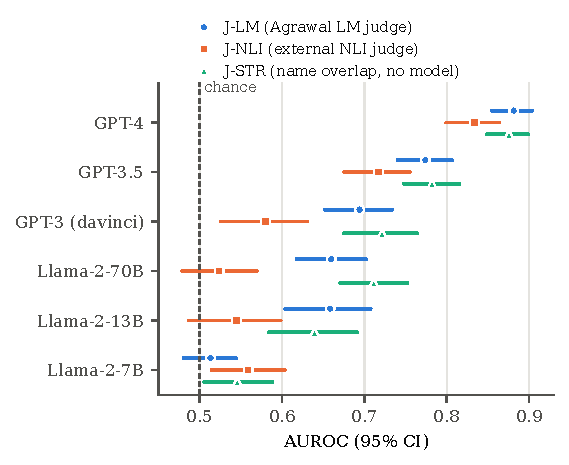
\includegraphics[width=0.62\linewidth]{figures/fig_e1_judges.pdf}
\Description{Dot plot with confidence intervals. For each of six models, three markers show the AUROC of the LM judge, the NLI judge and the name-overlap judge. GPT-4 is highest (about 0.83 to 0.88); Llama-2-7B is lowest, with all three judges between 0.51 and 0.56, near the dashed chance line at 0.5. The NLI judge is lowest for all models except Llama-2-7B.}
\caption{E1: AUROC of three judges applied to the same sampled author answers (190 main topics; 95\% topic-cluster bootstrap CIs). The dashed line marks chance.}
\label{fig:e1}
\end{figure}

\begin{table}[t]
\caption{E1: AUROC [95\% CI] per judge and paired differences from the LM judge. \textbf{Bold} differences have CIs that exclude 0. J-NLI-raw omits the refusal rule.}
\label{tab:e1}
\footnotesize
\setlength{\tabcolsep}{2.5pt}
\begin{tabular}{lccccc}
\toprule
Model ($n$, \%\,hall.) & J-LM & J-NLI & J-STR & J-NLI $-$ J-LM & J-STR $-$ J-LM \\
\midrule
GPT-4 (950, 48\%) & 0.881 [.855,.903] & 0.834 [.800,.864] & 0.876 [.849,.899] & \textbf{$-$0.047} [$-$.069,$-$.028] & $-$0.006 [$-$.016,.005] \\
GPT-3.5 (950, 61\%) & 0.774 [.740,.806] & 0.717 [.676,.755] & 0.782 [.748,.815] & \textbf{$-$0.057} [$-$.085,$-$.029] & +0.008 [$-$.005,.021] \\
GPT-3 (950, 74\%) & 0.694 [.652,.734] & 0.580 [.526,.630] & 0.722 [.675,.764] & \textbf{$-$0.114} [$-$.159,$-$.068] & \textbf{+0.027} [.008,.048] \\
Llama-2-70B (950, 66\%) & 0.660 [.618,.702] & 0.524 [.479,.569] & 0.711 [.671,.752] & \textbf{$-$0.136} [$-$.183,$-$.088] & \textbf{+0.052} [.027,.075] \\
Llama-2-13B (770, 77\%) & 0.658 [.604,.708] & 0.545 [.487,.598] & 0.640 [.584,.691] & \textbf{$-$0.113} [$-$.187,$-$.040] & $-$0.019 [$-$.069,.032] \\
Llama-2-7B (950, 69\%) & 0.513 [.481,.544] & 0.559 [.515,.603] & 0.546 [.506,.588] & +0.046 [$-$.003,.094] & +0.033 [$-$.021,.088] \\
\bottomrule
\end{tabular}
\end{table}

\textbf{H1 is not supported for any of the six registered contrasts.} On the Llama-2-7B main set ($n = 950$ references, 653 hallucinated), changing the judge did not restore performance for Llama-2-7B. All three judges remained close to chance, yielding AUROCs of 0.513 [0.481, 0.544] for the LM judge, 0.559 [0.515, 0.603] for the NLI judge, and 0.546 [0.506, 0.588] for name overlap. The paired difference between the NLI judge and the LM judge ($+0.046$ $[-0.003, +0.094]$) was not statistically significant. On the five larger models J-NLI is significantly \emph{worse} than the LM judge, by 0.047 to 0.136; no multiplicity correction was registered, so these are six separate 95\% intervals. The model-free J-STR is never significantly worse than J-LM and is significantly better on GPT-3 (+0.027) and Llama-2-70B (+0.052).

\textbf{Sensitivity.} Without the refusal rule, J-NLI on GPT-4 drops from 0.834 to 0.732, because consistent refusals look like agreement; for the other models the rule changes AUROC by at most 0.023. Using the 13B file with duplicates (V2) or without (E1) changes the 13B IQ AUC by 0.003.

\subsection{R1: ground-truth robustness}\label{sec:r1}
R1 covers 888 of the 950 Llama-2-7B main-set references (177 of 190 topics); the remaining 13 topics could not be queried before the OpenAlex daily limit was reached and are a contiguous block in the released file's order. Table~\ref{tab:r1} compares the labels. Excluding partial matches (27\% of references), agreement with Bing is $\kappa=0.72$ ($n=649$). The disagreement is asymmetric: Bing-hallucinated titles are almost never found in OpenAlex or Crossref (5 of 611), but 63 of 277 Bing-grounded titles (23\%) are not found either, consistent with exact-phrase web search ``grounding'' generic phrases that are not scholarly titles.

\begin{table}[t]
\caption{R1: Bing labels vs.\ the OpenAlex/Crossref oracle for Llama-2-7B (888 main-set references; $\tau=90$, partial $=[75,90)$).}
\label{tab:r1}
\small
\begin{tabular}{lcccc}
\toprule
Bing label & found & partial & not found & total \\
\midrule
grounded & 125 & 89 & 63 & 277 \\
hallucinated & 5 & 150 & 456 & 611 \\
\bottomrule
\end{tabular}
\end{table}

\textbf{Post-hoc label-noise check (not pre-registered).} To account for potential ground-truth errors in the original Bing labels, we ran a post-hoc label-noise check on a subset of 581 references from Llama-2-7B that were verified against scholarly databases. On this subset J-LM and J-NLI improved only modestly and J-STR did not improve, so all judges remained weak (J-LM 0.517 $\to$ 0.556 $[0.511, 0.604]$, J-NLI 0.556 $\to$ 0.613 $[0.551, 0.672]$, J-STR 0.548 $\to$ 0.538 $[0.471, 0.602]$, relative to the 888 R1 references; J-NLI $-$ J-LM $+0.057$ $[-0.012, 0.124]$). Label noise therefore explains part of the near-chance performance, but with confirmed labels the best judge is still weak and the NLI judge's advantage remains non-significant. The subset has only 125 grounded references, so its intervals are wide.

\subsection{RQ2: topic familiarity}\label{sec:rq2}
OpenAlex counts for the 190 leaf phrases range from 1{,}876 to 35.1 million works (median 1.08 million); the largest counts belong to generic words such as ``Design'' (35.1 million) and ``Availability'' (32.8 million), which illustrates the crudeness of the proxy. Figure~\ref{fig:rq2} shows the slopes. Five of six are negative (fewer fabrications on better-published topics), but \textbf{no model's CI excludes 0}, so H2 is not supported; the pooled slope with model fixed effects is $-0.144$ $[-0.342, 0.040]$. The clearest monotone pattern is Llama-2-13B (fabrication 81.8\%, 76.7\%, 72.7\% from low to high tertile; slope $-0.34$ $[-0.76, 0.02]$). Exploratory per-tertile AUROCs show no consistent dependence of detection quality on familiarity.

\begin{figure}[t]
\centering
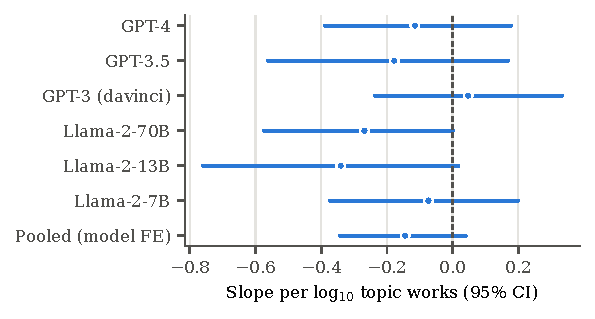
\includegraphics[width=0.62\linewidth]{figures/fig_rq2_slopes.pdf}
\Description{Forest plot of seven logistic slopes with confidence intervals: six models and a pooled estimate. Five point estimates are below zero, but every interval crosses the dashed zero line.}
\caption{RQ2: logistic slope of $P(\text{hallucinated})$ per $\log_{10}$ OpenAlex works of the topic (95\% topic-cluster bootstrap CIs). Negative means fewer fabrications on better-published topics.}
\label{fig:rq2}
\end{figure}

\section{Discussion}\label{sec:discussion}
\textbf{The judge is not the bottleneck at small scale.} If Llama-2-7B's author answers contained a consistency signal that its own judging failed to read, an independent judge should have exposed it. Neither a large DeBERTa NLI model nor exact token overlap does: all judges stay within 0.06 of chance. The answers themselves therefore appear to vary about as much for real references as for invented ones. This is consistent with the failure reported by \cite{agrawal2023hallucinating} lying in what the small model \emph{knows} about authorship rather than in how its consistency is assessed. Three alternatives remain open: (i) three samples may be too few to estimate consistency for a noisy generator; (ii) the decoding settings used to produce the released answers may suppress or exaggerate variation; (iii) label noise in the Bing ground truth could pull every judge towards chance. The post-hoc check in \S\ref{sec:r1} shows that (iii) accounts for some of the gap (judges reach 0.54--0.61 with confirmed labels) but not for most of it; (i) and (ii) require new generations, which this study did not run.

\textbf{Why NLI is the weakest judge.} A likely reason for NLI’s lower performance on author lists is that premise-hypothesis classifiers trained on standard text may label reordered or partially matching author names as neutral rather than contradictory, treating set-comparison tasks as unrelated statements. The model-free J-STR, which measures overlap directly, matches or beats the LM judge on every model. The more general lesson for consistency-based detection is that the agreement function should fit the answer type: SelfCheckGPT's NLI judge was designed for sentences of a biography, not for structured fields.

\textbf{Implications for research workflows.} A name-overlap check over three sampled author answers costs three short generations and no judge model, and is as informative as the LM judge. It remains a weak signal for small models, which supports the review's recommendation that citation existence be verified against bibliographic databases rather than inferred from the model's self-consistency.

\section{Limitations and Threats to Validity}\label{sec:limits}
\begin{itemize}[leftmargin=*]
  \item \textbf{Ground truth.} Labels are Agrawal et al.'s 2023 Bing exact-phrase searches. We evaluated them against OpenAlex and Crossref (R1), but only for Llama-2-7B and on 888 of 950 references, and this does not replace them. The label-agreement analysis is post hoc.
  \item \textbf{Scale.} Consistency checks fail at the 7B scale, but larger models such as Llama-2-13B and 70B are not at chance (LM-judge AUROC about 0.66), so consistency scoring is weak rather than non-functional as scale increases.
  \item \textbf{Fixed answers.} E1 isolates the judge by design; it cannot say whether different prompts or more samples would produce a usable signal at 7B. The planned new-generator experiment (Qwen2.5-1.5B, with direct, log-probability, verbal-confidence and SelfCheck detectors) was dropped after a measured cost of 334\,s per topic on the available hardware; its code is released but was not run on the main set.
  \item \textbf{Baseline scope.} The NLI baseline was validated by showing that our scorer is identical to the official implementation, not by re-measuring its published benchmark score.
  \item \textbf{Familiarity proxy.} Leaf-phrase search counts are crude: generic leaves such as ``Design'' count works far outside computing. RQ2 also performs six tests without correction.
  \item \textbf{Scope.} Computer-science topics, English, and closed or 2023-era models; J-STR's parser was tuned on pilot answers from these models.
\end{itemize}

\section{Reproducibility and AI Use}
The repository contains the frozen protocol, all decision and protocol-change records, the scripts that produce every table and figure from cached data, unit tests, environment logs and exact package versions. V2, E1 and RQ2 run from the released data on a laptop (E1: about one hour on an Apple-silicon GPU); R1 is limited by the OpenAlex and Crossref rate limits, and all API responses are cached so reruns need no network. AI assistance (Claude Code) was used for literature search, code generation, debugging and drafting; every AI-proposed source was checked against its primary page, every number in this paper comes from a logged run, and the AI-assistance log records the cases where verification changed the work, including an overclaimed novelty framing, a name parser that failed on real answer formats, and the auto-flip in the original AUC procedure.

\section{Conclusion}
Replacing the LM judge of a reference-consistency check with an external NLI model does not rescue detection for small models: on Llama-2-7B every judge stays near chance, and on larger models the NLI judge is worse than the LM it replaces. A model-free name-overlap judge is as good as the LM judge throughout. This is consistent with the small-model failure lying in the sampled answers rather than the judge. Future work should focus on testing citation verification across non-computer-science domains, evaluating newer small open models, exploring alternative decoding strategies, checking whether models support the specific claims made by cited works rather than just their existence, and verifying references against external bibliographic databases rather than relying solely on self-consistency.

\bibliographystyle{ACM-Reference-Format}
\bibliography{references}

\end{document}